187. \begin{figure}[ht!]
\center{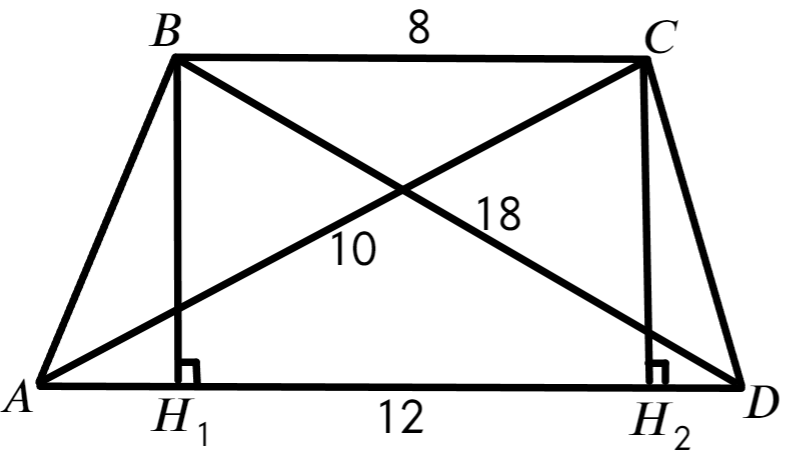
\includegraphics[scale=0.35]{g9-187.png}}
\end{figure}\\
Опустим высоты $BH_1=CH_2=h.$ Пусть $AH_1=x,$ тогда $H_2D=12-8-x=4-x$ и по теореме Пифагора для треугольников $ACH_2$ и $BDH_1$ имеем равенства
$h^2=100-(x+8)^2=324-(8+4-x)^2,$ откуда $100-x^2-16x-64=324-144+24x-x^2,\ 40x=-144.$ Этого быть не может, значит основание высоты $BH_1$ должно быть снаружи.\\
 \begin{figure}[ht!]
\center{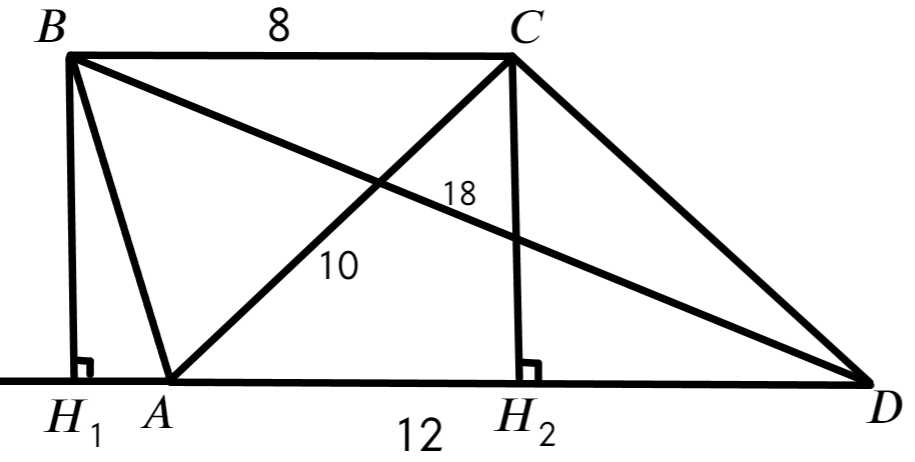
\includegraphics[scale=0.35]{g9-1871.png}}
\end{figure}\\
Опустим высоты $BH_1=CH_2=h.$ Пусть $AH_1=x,$ тогда $H_2D=12-(8-x)=4+x$ и по теореме Пифагора для треугольников $ACH_2$ и $BDH_1$ имеем равенства
$h^2=100-(8-x)^2=324-(12+x)^2,$ откуда $100-64+16x-x^2=324-144-24x-x^2,\ 40x=144,\ x=\cfrac{18}{5}.$ Тогда $h^2=100-\cfrac{484}{25}=\cfrac{2016}{25},\ h=\cfrac{12\sqrt{14}}{5}.$ Пусть расстояние от точки $D$ до прямой $AC$ равно $h_1.$ Посчитаем площадь треугольника $ADC$ двумя способами:
$\cfrac{1}{2}\cdot\cfrac{12\sqrt{14}}{5}\cdot12=
\cfrac{1}{2}\cdot h_1\cdot10,\ h_1=\cfrac{72\sqrt{14}}{25}.$\\
